\section{傅氏变换偏移方法的调整}
\label{sec:4.5}

我们首先要看一下如何对大于90°的倾角进行偏移,然后我们将着手解决Fourier变换偏
移方法的两个主要缺点,即这种方法的周期性质和这种方法容许速度空间可变的程度太低。

\subsection{倾角大于90°的情形}
\label{sec:4.5.1}

对大于90°的倾角进行偏移需要仔细处理指数式衰减的倏逝波能量(evanescent
energy
)。目前,大多数按深度进行外推的偏移程序对该种转成指数式衰减的倏逝波能量
都是忽略不计或是令其等于零。处置深度z上的倏逝波能量的正当办法应该是把这件事留给
向上进行第二次外推时去解决。在剖面的底部,下行波为零,从该剖面底部开始向上外推,
随着下行波的向上外推,所保存的倏逝波也就被恢复了。照例,所成映象是由时间$t
=0$时的波所形成的。

为解释说明这种概念,将草拟一个程序,该程序可作出两种映象,第一种是在反射面上
部的通常映象,第二种是在反射面下部的映象。对这些映象能够分别独立加以考虑或者把它
们相加。

该程序对速度作了简化约束。因为有这个假设,倏逝波能量可以被“原地”
贮存起来,直到反向外推之前都可以不去理它。值得注意的是第二次外推比第一次外推要节
省时间,因为永不出现倏逝波的区域$\mid k\mid<\mid \omega\mid/v(\tau_{max})$不需要处理。

\begin{figure}[H]
\centering
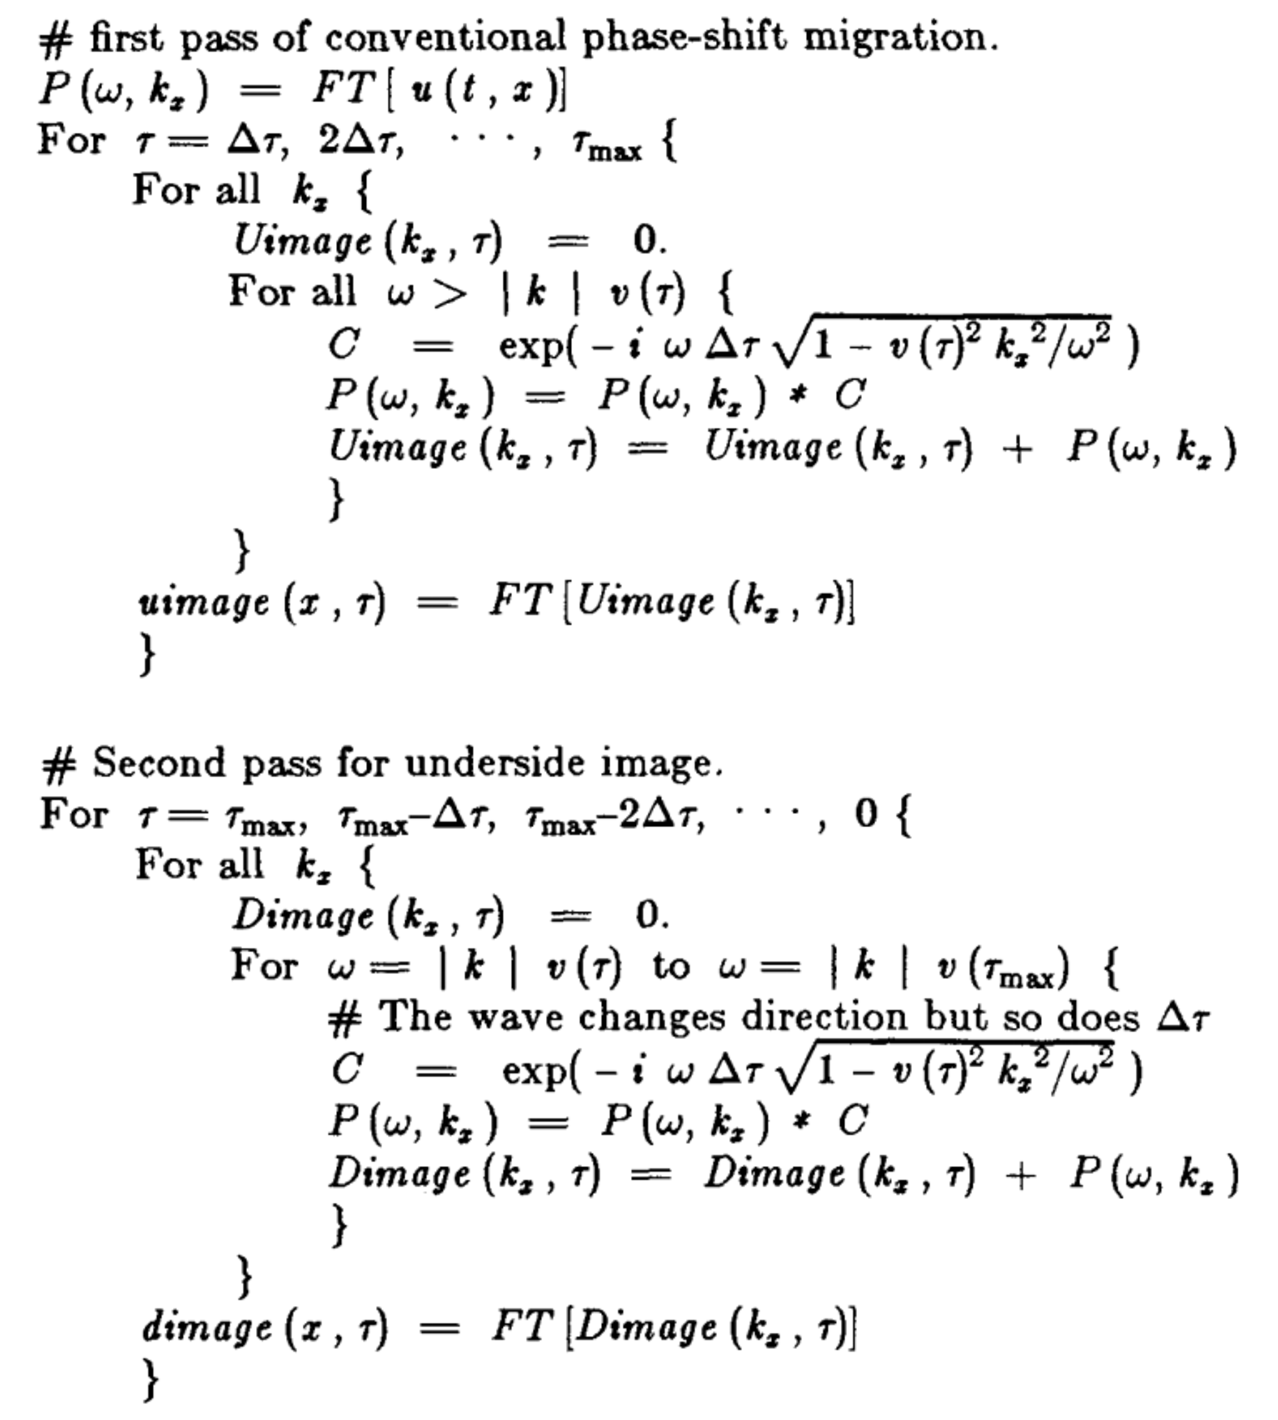
\includegraphics[width=0.65\textwidth]{crft/code1}
\caption[code1]{伪代码}
\label{fig:crft/code1}
\end{figure}

\subsection{防止相移偏移出现折叠现象(S.Levin, 1984) }
\label{sec:4.5.2}

图\ref{fig:crft/hyptrunc}表示一个双曲线族,注意,这些双曲线并未延展至无限大时间而是使它们在某
个截止时间$t_c$上截断。我们将阐述一种形成这类时间截断之数据的Fourier方法,该方法可
导致一种无折叠假象的相移偏移程序。

在开始采用快速傅氏变换算法时人们就已
注意到,可以将该算法应用于滤波处理。如果
将信号与滤波因子两端増补足够多的零值,那
就能够在周期性的Fourier变换域内准确地实
现瞬态滤波。同样的概念可应用于偏移处理,
如果在时间域与空间域内将野外数据和偏移双
曲线四周填补以足够多的零值,则在Fourier
变换域内就可以实现没有折叠现象的偏移,其
诀窍就是看如何能在Fourier变换域内构造出
图\ref{fig:crft/hyptrunc}中的各截断双曲线了。

\begin{figure}[H]
\centering
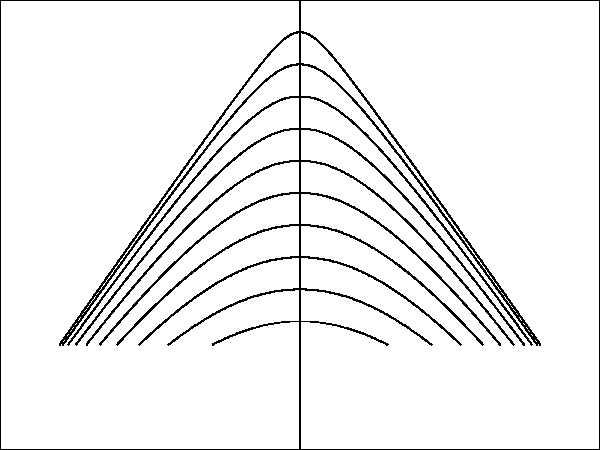
\includegraphics[width=0.65\textwidth]{crft/hyptrunc}
\caption[hyptrunc]{在某一特定时间上截断之双曲线}
\label{fig:crft/hyptrunc}
\end{figure}

为在时间L上截断,必须利用特殊的点源。震源越深,其张角(angular
aperture)就
必然越狭窄。使时间$t_0$上的初至之双曲线在某个时间$t_c$上被截断,在截止时间上之能量的传播
角度$\theta$由关系式$\cos\theta = t_0/t_c$给出,因而爆炸反射面就具有在$\sin\theta=vk_x/\omega$
时被截断的$k_x$谱。
一个90°的张角就是意味着具有无限大时间延迟的反射。下面是该程序的梗概:

\begin{figure}[H]
\centering
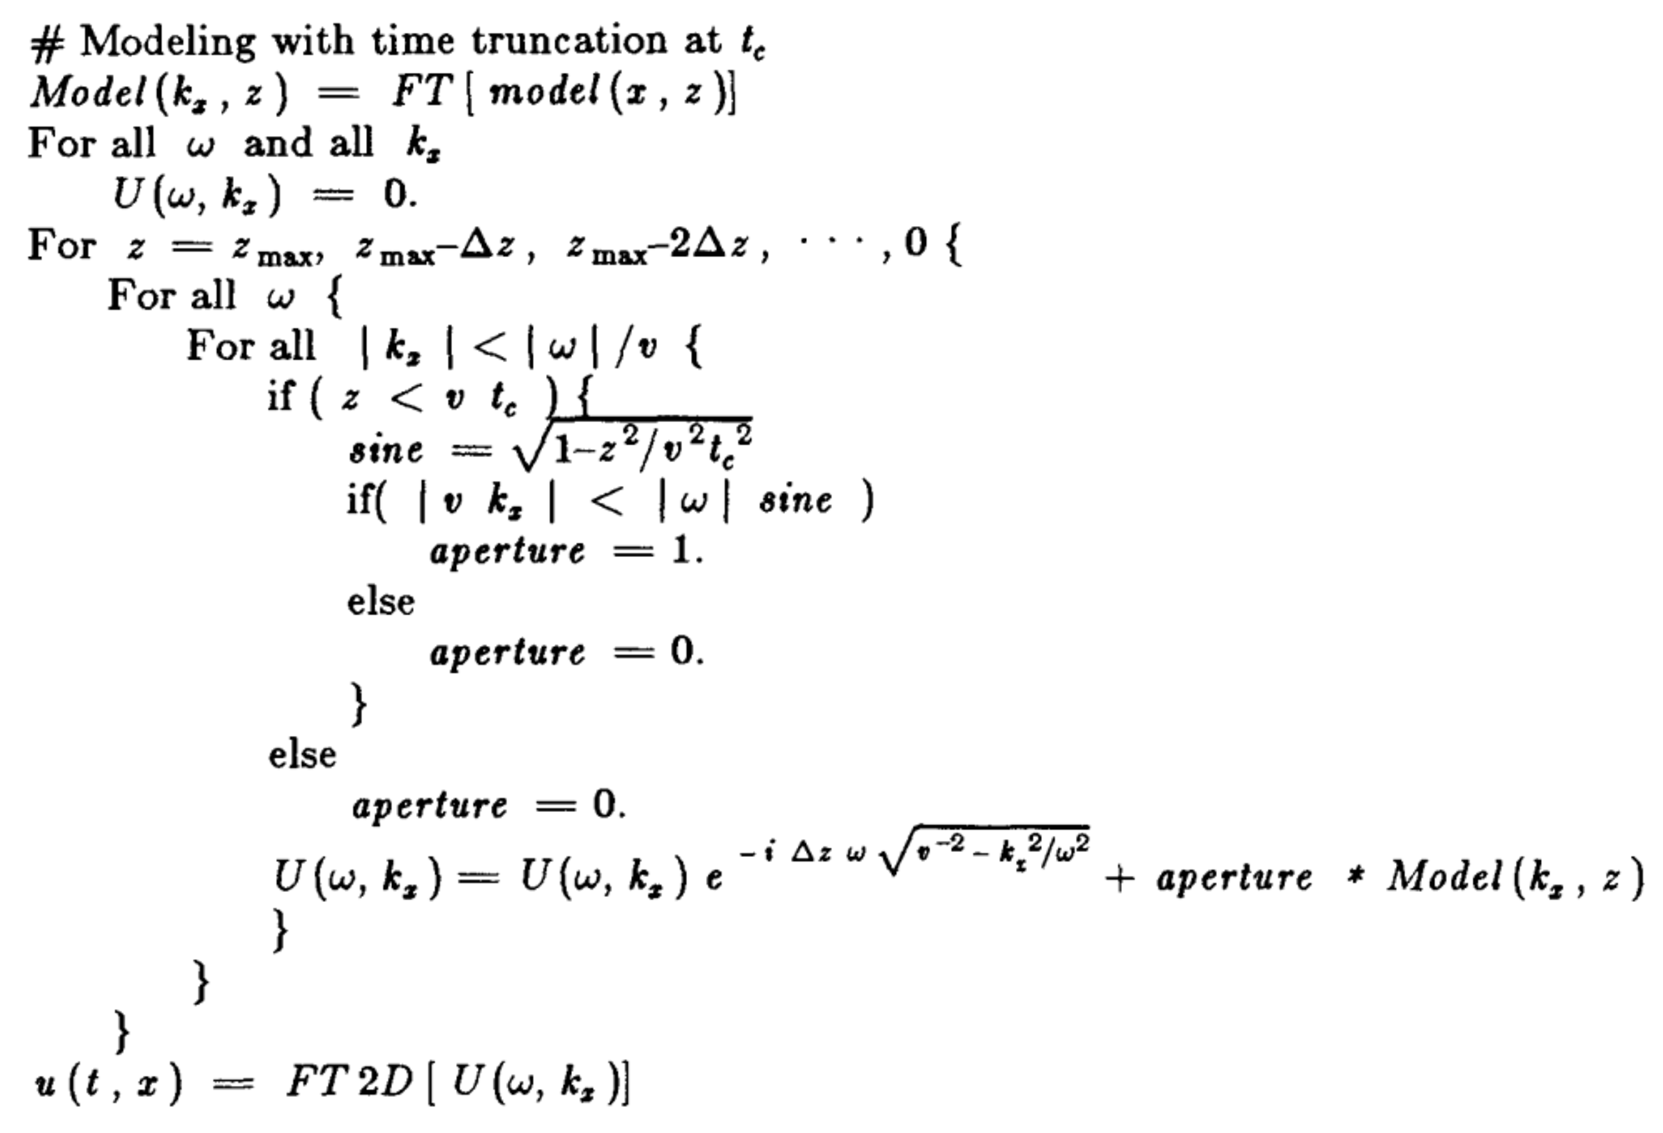
\includegraphics[width=0.65\textwidth]{crft/code2}
\caption[code2]{伪代码}
\label{fig:crft/code2}
\end{figure}

使深度$z$的循环迸行从浅至深的循环而不是从深至浅的循环,并且将向下延拓的数据乘以
孔径函数,就能够把上述模拟程序转变成偏移程序(参阅\ref{sec:1.3}节)。对程序进行这种修正不但
可改善偏移处理的质量,而且计算也较快速。


\subsection{控制Stolt偏移方法的折叠现象}
\label{sec:4.5.3}

像相移偏移算法一样,减少Stolt偏移算法计算假象的关键是必须压制时间域的折叠现
象,我们将要看到,这相当于是要进行精确的频率域内插。

首先,考虑在时间$t_0$上有一脉冲函数,其Fourier变换为$\exp(-i\omega t_0)$,当$t_0$很大时,这
时该Fourier变换是一个呈现迅速振荡的函数。迅速振荡之函数往往是难于内插的,最
好是对该时间函数进行后向时移(Shift backward
),从而起到将其频率函数进行平滑的
作用,然后对该频率函数进行内插,最后则取消时移使之恢复原状。设已知时间段$0<t<T$
上的地震数据,如将该数据时移至时间间隔$-T/2<t<T/2$,相应的频率函数就会被平滑。
因此,对Stolt偏移程序提出的第一个改进意见就是在频率域内乘以$\exp(i\omega T/2)$
,然后内插,最后再乘以$\exp(-i\omega T/2)$。

线性内插差不多是最容易实现的内插形式了。另一方面,Fourier变换理论则建议用
sinc函数作内插(根据定义$sinc u= (sinu)/u$)。
频率$\omega$的sinc函数反变换回时间域时是一
个时间t的矩形函数,在间隔$-T/2<t<T/2$上这个矩形函数取非零值。回想一下,快速逆
傅氏变换算法是在频率域内的均勻间隔上求和的,这隐含着各采样点之间应为零的假设,到
头来也就是假设时间域函数在给定的时间间隔之外是周期性的。现在令时间的矩形函数为时
间域内之乘因子,使该周期性时间函数转变为所观测的瞬态时间函数。在时间域内的这种乘
法等价于在频率域内采用适当的sinc函数所作的一种褶积。连续sinc函数与已知离散间隔的
频率函数作褶积实际就是内插。可惜,sinc函数是沿频率坐标轴无限延展的,更糟的是它衰
减很缓慢。所以,采用的是某种近似的或者截断的sinc函数。 Bill
Harlan曾诬明:斜坡衰减sinc函数达到令人满意的精度能比补零(zero padding)
更为节省计算时间。不过,事情
看来是,最好的办法还是应该既补零又采用某种sinc函数式的内插。Rosenbaum与Boudreaux
(1981年)的论文是有关内插问题的权威性研究。

\subsection{Stolt拉伸扩展法}
\label{sec:4.5.4}

采用深度方向的Fourier变换是Stolt偏移方法的一大长处,同时也是它的一大弱点。这是
一大长处是因为这使他的方法在运算上比所有其他方法都快速得多,这又是一个弱点是因为
它要求速度必须是深度的一种恒定函数。在地震剖面范围之内变化两倍是速度的典型变化范
围,而速度对偏移的影响则往往与速度的平方有关。为减轻这种困难,Stoit曾建议将时间
坐标轴拉伸扩展,使得数据看上去很像是由某一恒定速度的地层所产生的。
Stolt提出过下 列拉伸扩展函数:
\begin{subequations}
\begin{equation}
\tau(t)=(\frac{2}{v_0^2}\int_0^t t'v_{RMS}^2(t')dt')^{1/2}
\label{eq:ex4.5.1a}
\end{equation}
\begin{equation}
v_{RMS}^2(t)=\frac{1}{t}\int_0^t v^2(t')dt'
\label{eq:ex4.5.1b}
\end{equation}
\label{eq:ex4.5.1}
\end{subequations}

在涉及高速度的很大时间之处,Stolt的拉伸扩展意味着$\tau$值的增长要比t值快速一些。为能
应用快速傅氏变换FFT,要沿$\tau$轴均匀采样,这么一来,在很大时间之处,就得在t坐标轴上增大
采样密度;这正同关于地层Q值和采样定理的要求相反,但是大多数人都认为值得这么作。

导出式\ref{eq:ex4.5.1}的最直接方法是基于这么一种思想:要使理想双曲线顶部的曲率同拉
伸扩展之数据中的曲率相符一致。$(x,\tau)$ 空间内的理想双曲线方程为
\begin{equation}
v_0^2\tau^2=x^2+z^2
\label{eq:ex4.5.2}
\end{equation}
作简单的微分即可表明,双曲线顶部的曲率为
\begin{equation}
\frac{d^2\tau}{dx^2}\mid_{x=0}=\frac{1}{\tau v_0^2}
\label{eq:ex4.5.3}
\end{equation}
可以证明,除了速度必须用均方根速度代替之外
\begin{equation}
\frac{d^2 t}{dx^2}\mid_{x=0}=\frac{1}{tv_{RMS}^2}
\label{eq:ex4.5.4}
\end{equation}
式\ref{eq:ex4.5.3}是可应用于层状介质内的。我们现在要针对层状介质寻找出一种经拉伸扩展的
时间$\tau(t)$,使得可以用式\ref{eq:ex4.5.3}有效地代替式\ref{eq:ex4.5.4}。我们很想使$t(x)$曲线与
$(x)$曲线在所有$x$值情形下都能匹配,但那就会使问题过于复杂化了。退而求其次,我们
可以只求在双曲线顶部的导数能相符、即与$x=0$点上的$\tau[t(x)]$对$x$之二阶导数能够匹
配。代入式\ref{eq:ex4.5.3}与式\ref{eq:ex4.5.4}的关系,可由这种作法导出$\tau d\tau/dt$而的表达式。在进行
积分并取其平方根之后,即得出式\ref{eq:ex4.5.1}。

有一种与此不同的导出拉伸扩展时间$\tau$的方法,它可以在较陡角度时给出更精确的结
果,这种方法不是在顶点上使双曲线曲率匹配,而是在侧翼上离开顶部有若干距离之处使双
曲线斜率和函数值均匹配。实际偏移的正是双曲线的两翼而不是顶部,所以这种结果就要更
准确些。从代数运算说,这种导出方法也较容易,因为所需要的仅是一阶导数。对于任意深
度$z_i$上的反射面,将式\ref{eq:ex4.5.2}对$x$微分,得出
\begin{equation}
\frac{d\tau}{dx}=\frac{x}{\tau v_0^2}
\label{eq:ex4.5.5}
\end{equation}
在层状介质内也存在类似的表达式,为得出这个表达式,解出$x=\int v\sin\theta dt=p\int v^2 dt$,
就得出
$p=dt/dx$为:
\begin{equation}
\frac{dt}{dx}=\frac{x}{\int_0^tv^2(p,t)dt}
\label{eq:ex4.5.6}
\end{equation}
表达式\ref{eq:ex4.5.5}与\ref{eq:ex4.5.6}起着与式\ref{eq:ex4.5.3}和式\ref{eq:ex4.5.4}相同的作用,但式\ref{eq:ex4.5.5}与式\ref{eq:ex4.5.6}在任何地方均成立,而不仅只在双曲线顶部成立。对$\tau(t)$进行微分,得
\begin{equation}
\frac{d\tau}{dx}=\frac{d\tau}{dt}\frac{dt}{dx}
\label{eq:ex4.5.7}
\end{equation}
将式\ref{eq:ex4.5.5}与\ref{eq:ex4.5.6}代入式\ref{eq:ex4.5.7},得
\begin{equation}
\frac{x}{\tau v_0^2}=\frac{d\tau}{dt}\frac{x}{\int_0^tv^2(p,t)dt}
\label{eq:ex4.5.8}
\end{equation}
\begin{equation}
\tau d\tau=[\frac{1}{v_0^2}\int_0^tv^2(p,t')dt']dt
\label{eq:ex4.5.9}
\end{equation}
对式\ref{eq:ex4.5.9}进行积分,其左端得出$\tau^2/2$,这时取平方根即可得出式
\ref{eq:ex4.5.1a},但须采用下列均方根速度$v_{RMS}$的新定义
\begin{equation}
v_{RMS}^2=\frac{1}{t}\int_0^tv^2(p,t)dt
\label{eq:ex4.5.1c}
\end{equation}

现在的新鲜事是出现了Snell参量p。在以某种速度$v'(z)$为其特征的一种层状介质
内,$v(p,t)$定义为射线速度,该射线对地面呈某个角度,可用时差p量度。在实际处理
中,应该采用什么p值?最好的处理办法是先检查一下所用资料,针对你希望对它进行良好
偏移的那些同相轴测定出,$p=dt/dx$;有一个缺省值为
\begin{equation*}
p=\frac{2\sin30^{\circ}}{2.5km/s}=0.4ms/m
\end{equation*}
式中的因子2是根据爆炸反射面模型得出的。

\subsection{Gazdag的横向可变速度$v(x)$处理法}
\label{sec:4.5.5}

相移偏移方法很受欢迎,因为它允许速度随深度作任意变化,而且允许传播角度任意,
直至为90°。可惜,由于沿x坐标作Fourier变换,不允许速度有横向变化。为减轻这种困
难,JenoGazdag与Sguazzero(l984)提出过一种内插方法。回想一下\ref{sec:1.3}节内容,相移法
把数据$p(x,t)$通过二维Fourier变换,转换为$P(k_x,\omega)$,然后,乘以$\exp[ik_z(\omega,k_x)\Delta z]$
即可将$P(k_x,\omega)$按深度步长向下延拓。
Gazdag提出了若干个参考速度$v_1$、$v_2$、
$v_3$和$v_4$等,他用每一种速度向下延拓一个深度步长,获得经过向下延拓处理之数据的若干参
考结果$P_1$、$P_2$、$P_3$和$P_4$等,然后按横向波数$k_x$将每一种$P_i$作Fourier反变换,转换为
$p_i(x,\omega)$。在每一种x值时,他都对速度最相近的那些参考波进行了内插,得出最终值
$p(x,\omega)$。为下一个步长作准备,他把$p(x,\omega)$重又变换成$P(k_x,\omega)$,重复前面的
处理过程,就这样逐个步长作下去。由于对每一种参考速度情形都是重复通常的偏移计算,
这看来好像是一种效率不高的方法。使人惊奇的是,也许因为有利用阵列处理机进行计算所
具有的独特性质,这种方法似乎是很成功的。

\subsection{习 题}
\label{sec:4.5.6}

\begin{enumerate}
\item 为在时间$t_c$获得尖锐的截止,就需要频率域内的谱具有宽广频带。设已知图\ref{fig:crft/hyptrunc}是在一种$1000\times
1000$的网格上表示的,试推断出在截止时间$t^c$内的不确定度(uncertainty)。
\item 因为对时间t的Fourier变换具有周期性,相移方法往往产生对$z$轴是周期性的偏移。通
常,这并不引起麻烦,因为我们不理会很大的$z$很大深度上的上行波在$t=0$
以前应该是等
于零的。Kjartansson曾指出,如果在继续往下进行计算之前,从波场中减掉在$t=0$时的
波,那就可以避免沿深度$z$的周期性,因而信息永不可能与负时间和“折叠”现象沾边。试
指出应如何改变相移方法的程序。
\end{enumerate}

